\documentclass[12pt,a4paper]{article}

\usepackage[T2A]{fontenc}
\usepackage[utf8]{inputenc}
\usepackage[russian]{babel}

\usepackage{amsmath}
\usepackage{amssymb}
\usepackage{geometry}
\usepackage{graphicx}
\usepackage{hyperref}
\usepackage{indentfirst}
\usepackage{float}

\geometry{
left=25mm,
right=25mm,
top=25mm,
bottom=25mm
}

\title{
Историческое развитие методов скелетизации изображений:\\
от Medial Axis Transform к алгоритмам утончения изображений
}

\author{}
\date{}

\begin{document}

\maketitle

\section{Введение}

Скелетизация является одной из классических задач цифровой обработки изображений и компьютерного зрения. Ее цель состоит в построении компактного представления объекта, сохраняющего его основные геометрические и топологические свойства. Вместо хранения всей области изображения используется множество точек, отражающих внутреннюю структуру объекта и его характерные особенности.

Исторически развитие методов скелетизации связано с задачами анализа формы объектов и распознавания образов. Одной из наиболее влиятельных работ в данном направлении стала работа Гарри Блума, предложившего аппарат Medial Axis Transform, далее $MAT$ \cite{blum1967}. В дальнейшем идеи $MAT$ оказали существенное влияние на развитие методов утончения изображений и современных алгоритмов скелетизации \cite{lam1992}.

\section{Прикладная задача анализа формы объектов}

В ранних системах распознавания образов исследователей интересовала не столько сама форма объекта, сколько возможность выделить признаки, позволяющие сравнивать различные объекты между собой.

Например, при анализе символов важно определить:

\begin{itemize}
	\item количество ветвлений;
	\item число конечных точек;
	\item наличие замкнутых областей;
	\item взаимное расположение частей объекта;
	\item локальную толщину различных участков.
\end{itemize}

Хранение полного контура объекта требует большого объема данных и затрудняет выделение подобных признаков. Поэтому возникла задача построения более компактного представления формы объекта \cite{blum1967}.

\section{Работа Блума 1967 года}

В работе \cite{blum1967} Блум предложил описывать форму объекта через его внутреннюю структуру.

Основная идея состояла в том, что для распознавания формы важна не только граница объекта, но и расположение его центральных осей. Для формального описания этой идеи был введен аппарат $MAT$.

Скелет объекта определяется через множество центров максимальных вписанных окружностей. Такое представление позволяет одновременно хранить информацию о структуре объекта и его локальной толщине.

\section{Мотивация автора и постановка задачи}

В работе \cite{blum1967} Блум рассматривает проблему описания формы объектов с точки зрения распознавания образов и биологического зрения. Основной вопрос заключается в том, каким образом можно представить форму объекта так, чтобы сохранить наиболее важную информацию о его структуре и одновременно избавиться от избыточных деталей границы.

Автор отмечает, что непосредственное описание объекта через его контур далеко не всегда удобно. Контур может содержать большое количество точек и быть чувствительным к шуму, локальным деформациям и особенностям дискретизации. При этом для распознавания объектов зачастую более важными оказываются внутренние симметрии формы, точки ветвления, локальная толщина различных частей объекта и взаимное расположение его элементов.

С точки зрения Блума форма объекта определяется не только его внешней границей, но и организацией внутренних геометрических отношений между различными частями объекта. Именно это наблюдение послужило основой для введения Medial Axis Transform.

\section{Формальное определение Medial Axis Transform}

Пусть объект представлен областью
\[
A \subset \mathbb{R}^{2}.
\]

Граница объекта обозначается через
\[
\partial A.
\]

Рассмотрим замкнутый круг радиуса $r$ с центром в точке $x$:
\[
B(x,r)=
\{y\in\mathbb{R}^{2}\mid \|x-y\|\le r\}.
\]

Круг называется вписанным в объект, если
\[
B(x,r)\subseteq A.
\]

Максимальным вписанным кругом называется такой круг $B(x,r)$, для которого не существует круга $B(x',r')$, удовлетворяющего условиям
\[
B(x,r) \subset B(x',r') \subseteq A,
\qquad
B(x,r) \ne B(x',r').
\]

Иначе говоря, максимальный вписанный круг нельзя увеличить или вложить в другой больший вписанный круг, не выйдя за пределы объекта.

Medial Axis определяется как множество центров всех максимальных вписанных кругов \cite{blum1967}. Более формально:
\[
M(A)=
\left\{
x\in A
\mid
x
\text{ является центром максимального вписанного круга}
\right\}.
\]

На практике используется более богатое представление:
\[
MAT(A)=
\{
(x,r)
\mid
x\in M(A),
\; r = d(x,\partial A)
\}.
\]

Таким образом каждая точка скелета хранит не только свое положение, но и радиус соответствующего максимального вписанного круга.

\subsection{Свойство восстановления объекта}

Одним из важнейших свойств $MAT$ является возможность восстановления исходного объекта.

Пусть известны все элементы множества $MAT(A)$. Тогда объект может быть восстановлен как объединение соответствующих максимальных кругов:
\[
A=
\bigcup_{(x,r)\in MAT(A)}
B(x,r).
\]

Следовательно, $MAT$ представляет собой не просто описание формы объекта, а альтернативный способ хранения самой области \cite{blum1967}.

\section{Основные идеи и аргументы Блума}

В статье \cite{blum1967} автор приводит несколько аргументов в пользу использования Medial Axis Transform как базового описания формы объекта.

Во-первых, скелет позволяет существенно уменьшить объем данных, необходимых для хранения формы. Вместо хранения полного контура объекта достаточно хранить его центральную структуру и радиусы максимальных вписанных окружностей.

Во-вторых, Medial Axis содержит информацию о локальной толщине объекта. Каждой точке скелета соответствует радиус максимальной вписанной окружности, что позволяет описывать не только структуру объекта, но и его размеры.

В-третьих, Medial Axis Transform сохраняет достаточное количество информации для восстановления исходного объекта. Благодаря этому MAT можно рассматривать не просто как набор признаков, а как альтернативную форму представления геометрического объекта.

Наконец, автор отмечает, что точки ветвления скелета естественным образом соответствуют характерным особенностям формы и могут использоваться для последующего анализа и распознавания объектов.

\begin{figure}[H]
	\centering
	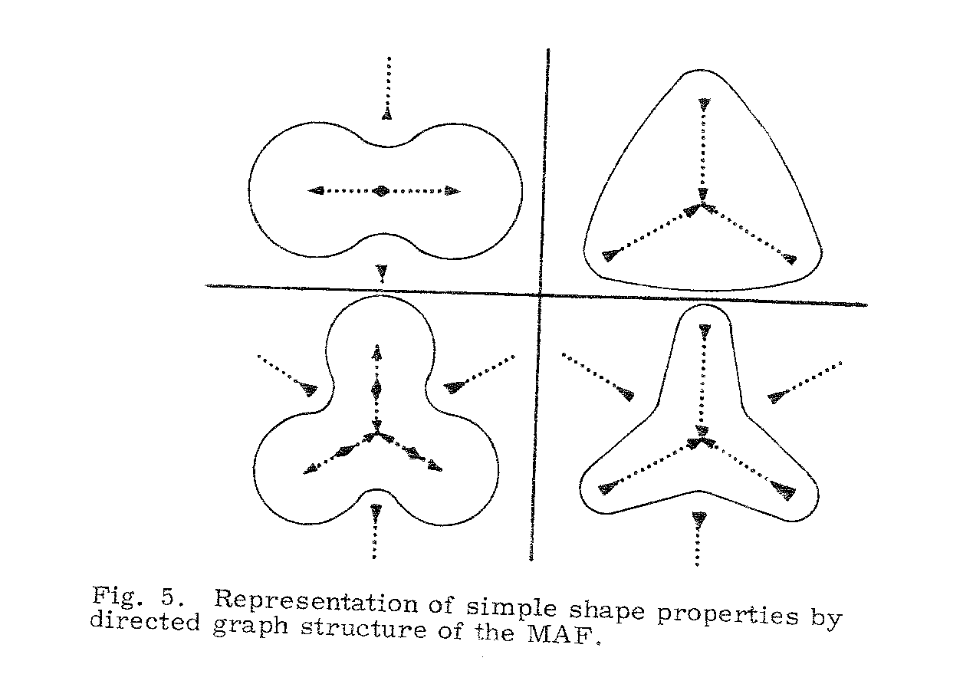
\includegraphics[width=\textwidth]{images/simple_shape.png}
	\caption{Представление простых геометрических фигур через структуру medial axis. Ветви и узлы скелета отражают основные геометрические свойства формы объекта}
	\label{fig:simple_shape}
\end{figure}

\begin{figure}[H]
	\centering
	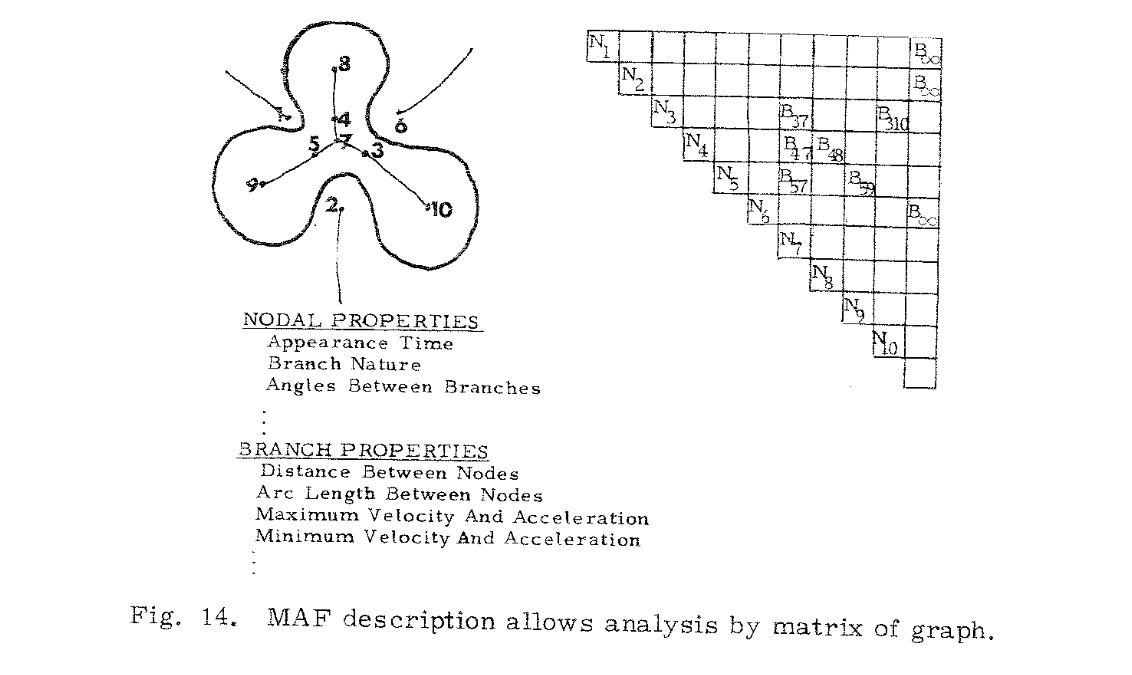
\includegraphics[width=0.9\textwidth]{images/matrix_graph.png}
	\caption{Использование medial axis для построения графового описания формы объекта. Узлы графа соответствуют характерным точкам скелета, а ветви описывают взаимосвязь различных частей объекта}
	\label{fig:matrix_graph}
\end{figure}

\section{Модель распространения фронта}

Для интуитивного объяснения Medial Axis Блум предложил модель распространения фронта, известную как grassfire model \cite{blum1967}.

Представим, что вся граница объекта одновременно поджигается. Фронт огня начинает распространяться внутрь области с постоянной скоростью
\[
v=1.
\]

Расстояние от точки $x$ до границы определяется как
\[
d(x,\partial A)=
\inf_{y\in\partial A}
\|x-y\|.
\]

Положение фронта в момент времени $t$ можно описать множеством точек
\[
F(t)=
\{
x\in A
\mid
d(x,\partial A)=t
\}.
\]

Когда два или более фронта сталкиваются, образуются точки скелета. Таким образом скелет можно рассматривать как множество точек столкновения фронтов распространения.

Данная модель связывает геометрическую структуру объекта с расстоянием до его границы и естественным образом приводит к понятию distance transform.

\begin{figure}[H]
	\centering
	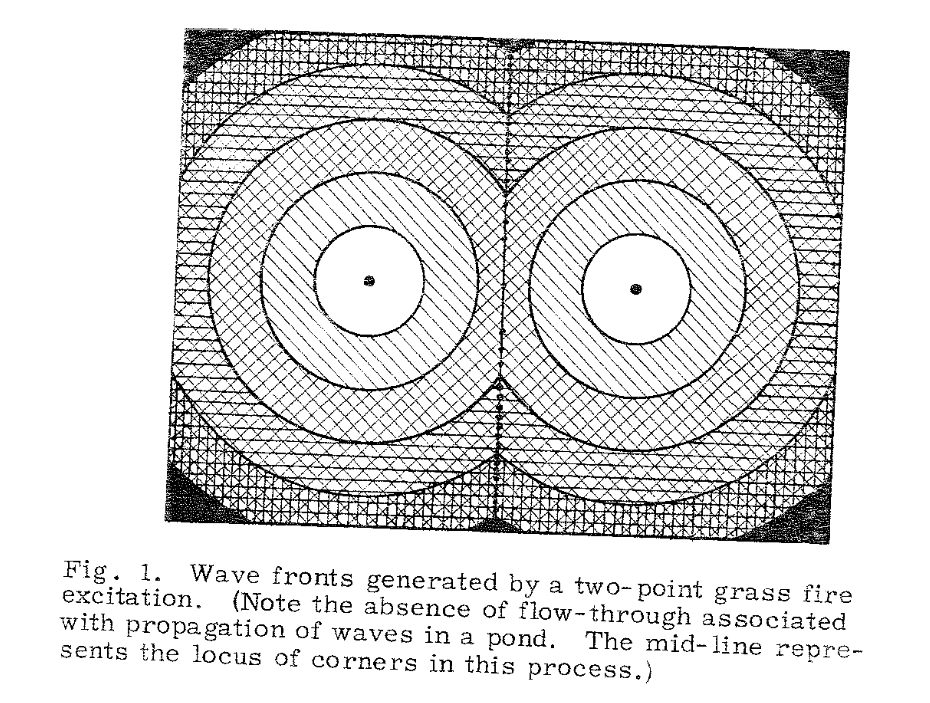
\includegraphics[width=\textwidth]{images/grassfire.png}
	\caption{Формирование medial axis как множества точек столкновения фронтов распространения}
	\label{fig:grassfire}
\end{figure}

\begin{figure}[H]
	\centering
	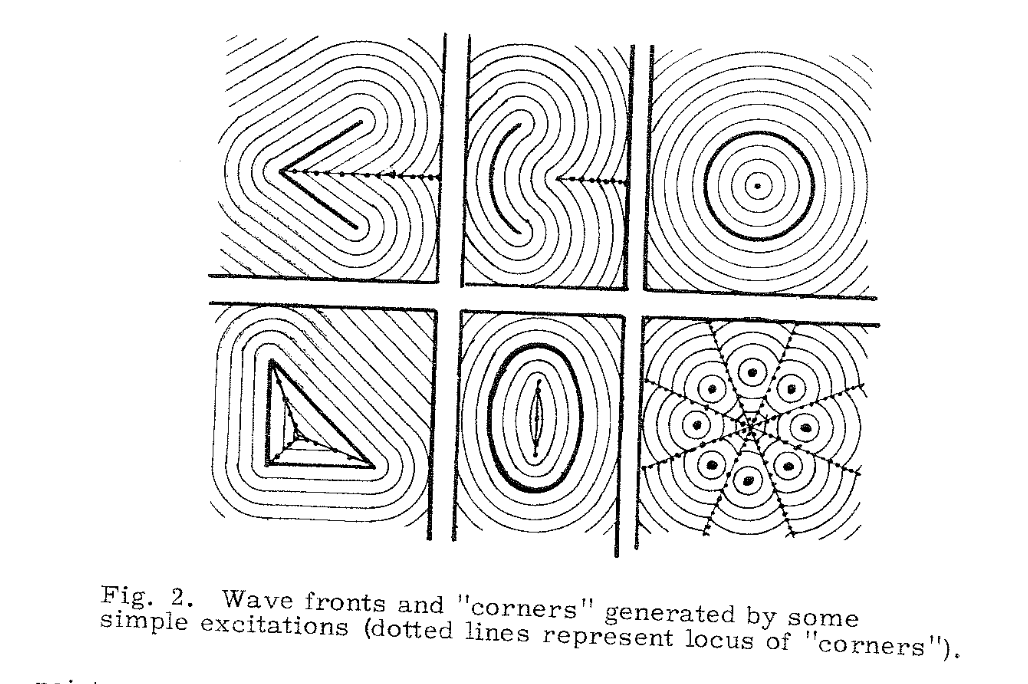
\includegraphics[width=\textwidth]{images/wavefronts.png}
	\caption{Примеры распространения фронтов для различных геометрических фигур. Пунктирными линиями показаны траектории особых точек, формирующих структуру medial axis}
	\label{fig:wavefronts}
\end{figure}

\section{Примеры из оригинальной статьи}

В работе \cite{blum1967} приведен ряд примеров объектов различной формы, для которых строится Medial Axis. Среди них встречаются как простые геометрические фигуры, так и более сложные биологические формы.

Во всех примерах демонстрируется одна и та же идея. Для каждой точки скелета существует максимальная вписанная окружность, касающаяся границы объекта как минимум в двух точках. По мере изменения радиуса и положения окружности формируется центральная структура объекта.

Особый интерес представляют объекты с ветвлениями. В таких случаях ветви скелета естественным образом соответствуют ветвям исходного объекта. Это позволяет использовать Medial Axis для описания структуры объектов сложной формы.

\begin{figure}[H]
	\centering
	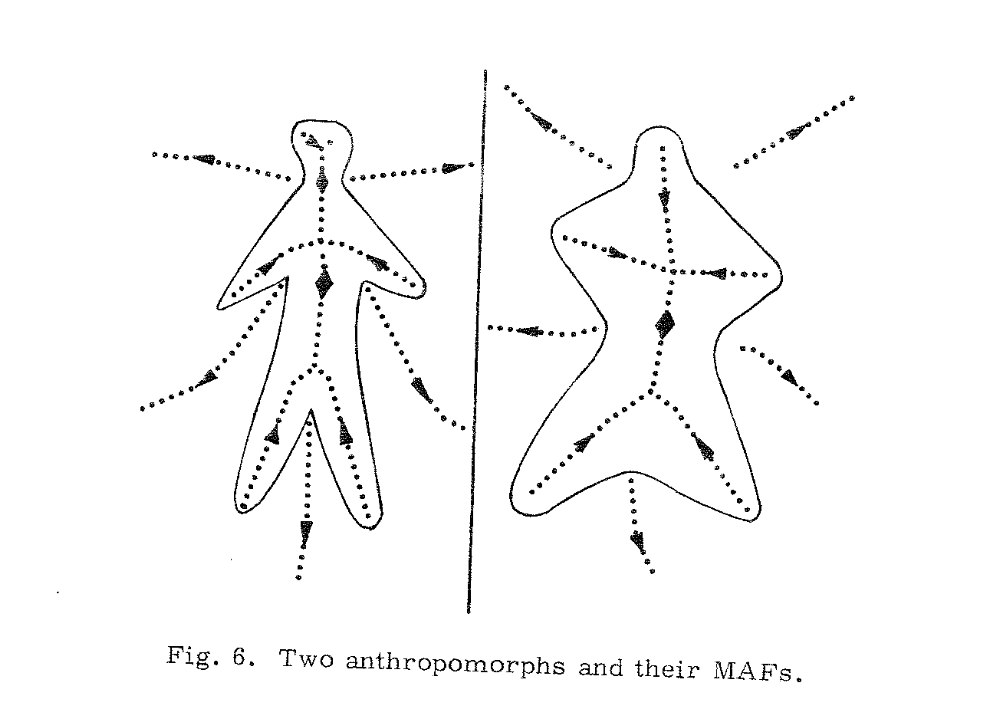
\includegraphics[width=\textwidth]{images/complex_shape.png}
	\caption{Примеры сложных объектов и соответствующих им medial axis. Скелет сохраняет основную структуру формы и позволяет выделять характерные части объекта}
	\label{fig:complex_shape}
\end{figure}

\section{Distance Transform}

Для точки $x\in A$ определим расстояние до границы объекта:
\[
D(x)
=
\min_{y\in\partial A}
\|x-y\|.
\]

Функция
\[
D:A\rightarrow\mathbb{R}
\]
называется функцией расстояния или distance transform. Она показывает, насколько каждая внутренняя точка удалена от ближайшей точки границы.

В цифровой обработке изображений используются различные метрики.

Евклидова метрика:
\[
\rho_2((i,j),(u,v))
=
\sqrt{
	(i-u)^2+
	(j-v)^2
}.
\]

Манхэттенская метрика:
\[
\rho_1((i,j),(u,v))
=
|i-u|+
|j-v|.
\]

Шахматная метрика:
\[
\rho_\infty((i,j),(u,v))
=
\max
\left(
|i-u|,
|j-v|
\right).
\]

В зависимости от выбранной метрики получаются различные варианты distance transform.

\begin{figure}[H]
	\centering
	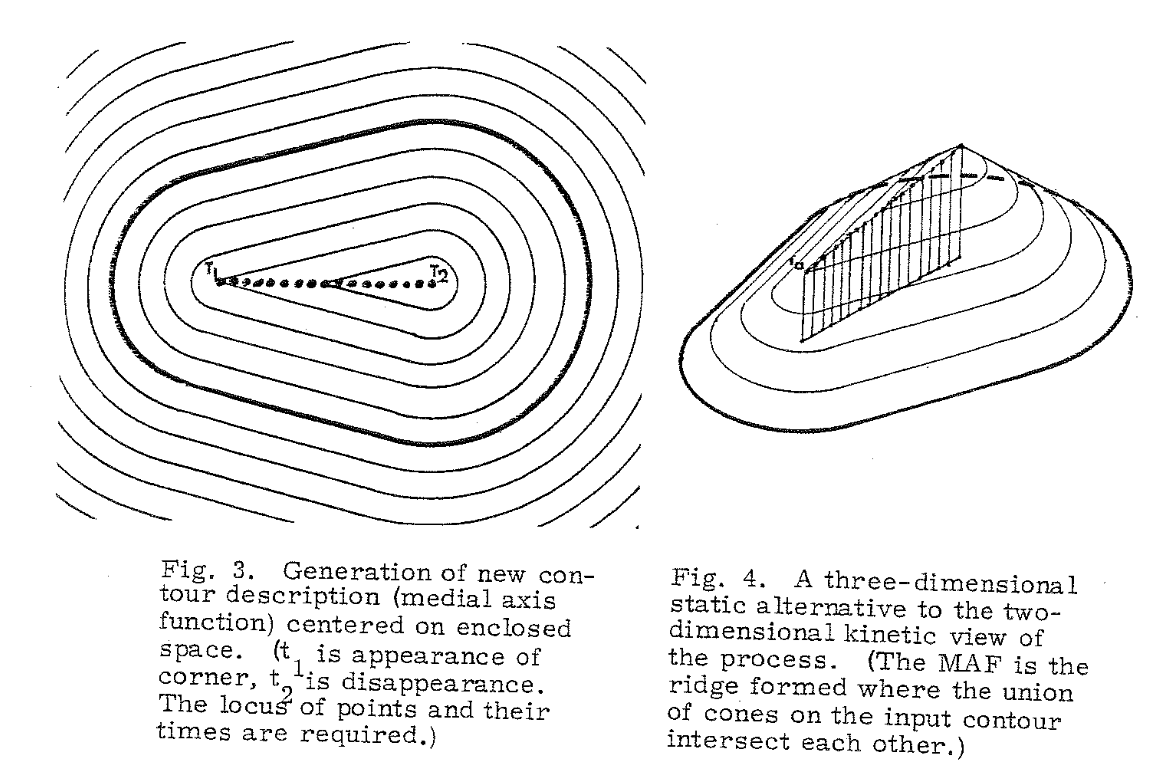
\includegraphics[width=\textwidth]{images/new_contour.png}
	\caption{Связь функции расстояния и medial axis. Линии равного расстояния до границы образуют фронты распространения, а их особенности формируют скелет объекта}
	\label{fig:new_contour}
\end{figure}

\section{Связь Distance Transform и Medial Axis}

Distance Transform и Medial Axis тесно связаны между собой.

Рассмотрим функцию расстояния

\[
D(x)
=
\min_{y\in\partial A}
\|x-y\|.
\]

Значение функции возрастает по мере удаления от границы объекта. Максимумы функции расстояния располагаются в центральных областях фигуры.

В непрерывном случае точки Medial Axis соответствуют особенностям функции расстояния. В цифровом случае это приводит к естественной идее поиска локальных максимумов карты расстояний.

Пусть

\[
N(p)
\]

обозначает множество соседей пикселя \(p\).

Тогда пиксель можно рассматривать как принадлежащий скелету, если

\[
D(p)
\ge
D(q)
\qquad
\forall q\in N(p).
\]

Именно эта идея лежит в основе многих практических алгоритмов построения скелета через distance transform.

\section{Дискретизация Medial Axis}

В цифровом случае изображение представляется множеством пикселей
\[
A\subseteq \mathbb{Z}^2.
\]

Для каждого пикселя вычисляется расстояние до ближайшего граничного пикселя:
\[
D(i,j)
=
\min_{(u,v)\in \partial A}
\rho((i,j),(u,v)).
\]

После построения карты расстояний скелет может быть найден как множество локальных максимумов функции расстояния.

Пусть $N(p)$ обозначает множество соседей пикселя $p$. Тогда пиксель считается принадлежащим скелету, если
\[
D(p)
\ge
D(q)
\qquad
\forall q\in N(p).
\]

Такой подход непосредственно следует из модели распространения фронта и является одной из простейших дискретных реализаций идеи Блума.

\section{Последовательная обработка цифровых изображений}

Параллельно с работами Блума развивались методы цифровой обработки изображений, ориентированные на последовательные операции над пикселями.

Одной из наиболее известных работ данного периода является статья Rosenfeld и Pfaltz \cite{pfaltz1966}. Авторы рассматривают цифровое изображение как дискретную структуру и показывают, каким образом различные характеристики изображения могут вычисляться посредством локальных операций над соседними пикселями.

Особое внимание уделяется вопросам связности, распространения меток и построения различных характеристик изображения посредством последовательных проходов по пикселям.

Подобный подход оказал существенное влияние на развитие алгоритмов обработки изображений и во многом определил направление дальнейших исследований в области distance transform, скелетизации и выделения связных компонент.

\section{Особенности вычислительной техники эпохи}

Ранние исследования в области обработки изображений выполнялись на мэйнфреймах и специализированных вычислительных системах.

Было бы неверно утверждать, что вычислительных ускорителей не существовало вовсе. Однако отсутствовали современные программируемые графические процессоры и массовые параллельные вычисления.

Основными ограничениями являлись:

\begin{itemize}
	\item высокая стоимость памяти;
	\item ограниченный объем оперативной памяти;
	\item необходимость последовательной обработки изображений;
	\item высокая стоимость хранения промежуточных структур данных.
\end{itemize}

Поэтому ранние алгоритмы ориентировались на локальные операции над пикселями и последовательные проходы по изображению \cite{pfaltz1966}.

\section{Ограничения Medial Axis Transform}

Несмотря на привлекательность геометрической интерпретации, Medial Axis Transform обладает рядом недостатков.

Наиболее известной проблемой является чувствительность к шуму. Даже небольшое локальное изменение границы объекта может привести к появлению новой ветви скелета.

Кроме того, скелет может существенно изменяться при незначительных деформациях формы объекта. Такая нестабильность затрудняет использование MAT в практических задачах анализа изображений.

Еще одной проблемой является сложность точного вычисления Medial Axis в дискретном случае. Определение максимальных вписанных окружностей естественно формулируется в непрерывном пространстве, тогда как реальные изображения представлены на дискретной решетке пикселей.

Указанные ограничения стали одной из причин появления альтернативных методов скелетизации.

\section{Переход к алгоритмам утончения}

Несмотря на привлекательность геометрической интерпретации $MAT$, его практическое применение столкнулось с рядом трудностей.

Даже небольшие изменения границы могут приводить к возникновению большого количества дополнительных ветвей скелета. Данная проблема подробно обсуждается в обзоре \cite{lam1992}.

Поэтому в дальнейшем получили развитие алгоритмы утончения, или thinning.

Основная идея thinning заключается в последовательном удалении граничных пикселей при сохранении связности объекта.

Наиболее известным представителем данного класса методов является алгоритм Zhang-Suen \cite{zhangsuen1984}. Он использует локальные правила удаления пикселей и постепенно преобразует объект в одно-пиксельный скелет. Вместо поиска максимальных вписанных окружностей выполняется последовательное удаление граничных пикселей по локальным правилам. Такой подход значительно проще реализуется на цифровых изображениях и лучше соответствует вычислительным ограничениям эпохи.

Алгоритмы утончения можно рассматривать как попытку сохранить основные преимущества Medial Axis Transform и одновременно избавиться от его недостатков.

Фактически алгоритмы утончения можно рассматривать как дискретное развитие первоначальных идей $MAT$.

\section{Заключение}

Предложенный Блумом аппарат $MAT$ стал одним из первых формальных способов описания формы объектов через их внутреннюю структуру.

Основу метода составляют понятия максимальных вписанных кругов, distance transform и модель распространения фронта. Несмотря на ограничения вычислительной техники 1960-х годов, предложенные идеи оказались чрезвычайно плодотворными и оказали значительное влияние на дальнейшее развитие методов обработки изображений.

В дальнейшем развитие данного направления привело к появлению алгоритмов утончения, многие из которых используются и сегодня \cite{zhangsuen1984,lam1992}.

\begin{thebibliography}{99}
	
	\bibitem{blum1967}
	Blum H.
	A Transformation for Extracting New Descriptors of Shape //
	Models for the Perception of Speech and Visual Form.
	MIT Press, 1967.
	pp. 362--380.
	
	\bibitem{pfaltz1966}
	Rosenfeld A., Pfaltz J. L.
	Sequential Operations in Digital Picture Processing //
	Journal of the ACM.
	1966.
	Vol. 13, No. 4.
	pp. 471--494.
	
	\bibitem{zhangsuen1984}
	Zhang T. Y., Suen C. Y.
	A Fast Parallel Algorithm for Thinning Digital Patterns //
	Communications of the ACM.
	1984.
	Vol. 27, No. 3.
	pp. 236--239.
	
	\bibitem{lam1992}
	Lam L., Lee S.-W., Suen C. Y.
	Thinning Methodologies -- A Comprehensive Survey //
	IEEE Transactions on Pattern Analysis and Machine Intelligence.
	1992.
	Vol. 14, No. 9.
	pp. 869--885.
	
\end{thebibliography}

\end{document}